% !TEX program = xelatex
\documentclass[a4paper, UTF8, fontset=adobe]{ctexart}

\usepackage[left=2.50cm, right=2.50cm, top=2.50cm, bottom=2.50cm, headheight=14pt]{geometry}

\usepackage[unicode=true,colorlinks,urlcolor=blue,linkcolor=blue,bookmarksnumbered=true]{hyperref}
\usepackage{latexsym,amssymb,amsmath,amsbsy,amsopn,amstext,amsthm,amsxtra,color,bm,calc,ifpdf}
\usepackage{graphicx}
\usepackage{enumerate}
\usepackage{fancyhdr}
\usepackage{listings}
\usepackage{multirow}
\usepackage{makeidx}
\usepackage{xcolor}
\usepackage{fontspec}
\usepackage{subfigure}
\usepackage{pythonhighlight}

\pagestyle{fancy}
\fancyhead[L]{}
\fancyhead[C]{Formula Derivation of R-VIO}
\fancyhead[R]{}

\begin{document}
	
\tableofcontents

\thispagestyle{empty}

\newpage

\begin{figure}
\centering
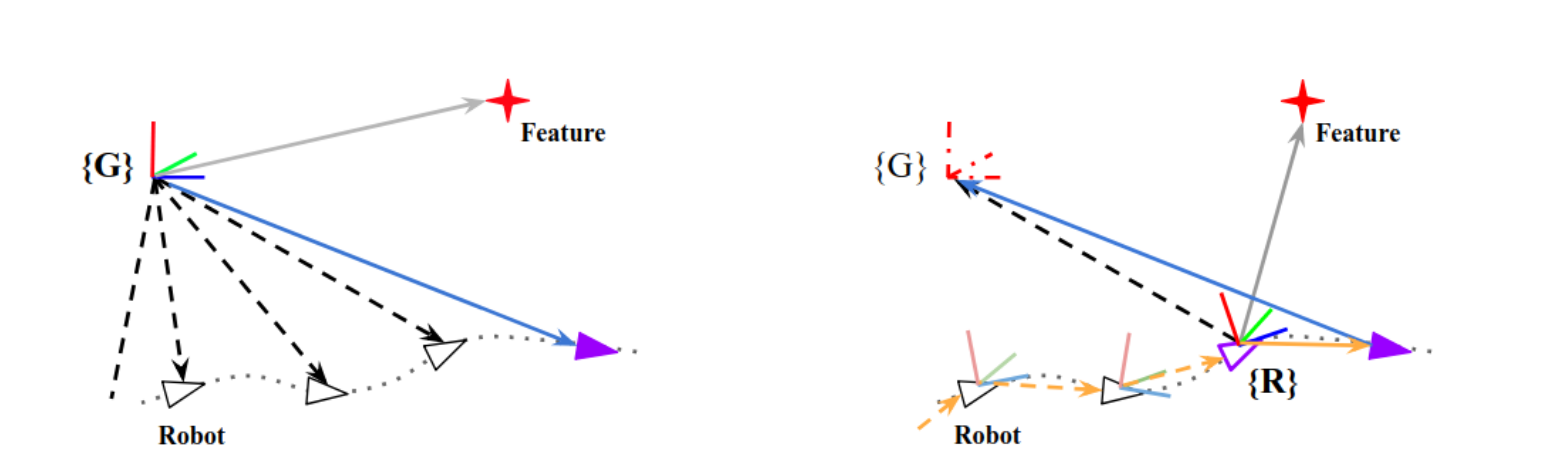
\includegraphics[width=0.65\textwidth]{figures/robocentric formulation illustration.png}
\caption{Figure 1.1: World-centric vs. robocentric formulation}
\end{figure}

\section{引言}

在此填写引言

\

\section{第2章标题}

以下是一些样例:

\textbf{加粗文本}

\textit{倾斜文本}

\underline{下划线文本}

项目编号:

\begin{itemize}
    \item XXX
    \item XXX
    \item XXX
\end{itemize}

\begin{enumerate}
    \item XXX
    \item XXX
    \item XXX
\end{enumerate}

行内公式:$\int_a^b f(x)dx = F(b)-F(a)$

另起一行的公式:
\begin{equation}
    \int_a^b f(x)dx = F(b)-F(a)
\end{equation}

插入图片:([scale=] 中的数可以控制图片大小;后面的括号表示图片的路径,请把图片上传到figures文件夹中;caption表示图片的标题)



插入表格:
\begin{tabular}{|c|c|}% 通过添加 | 来表示是否需要绘制竖线
\hline  % 在表格最上方绘制横线
(1,1)&(1,2)\\
\hline  %在第一行和第二行之间绘制横线
(2,1)&(2,2)\\
\hline % 在表格最下方绘制横线
\end{tabular}

\subsection{小节}

在此填写小节内容

\subsubsection{小小节}

在此填写小小节内容

\

\section{结论}

在此填写结论

\

\

\section*{参考文献}

在此填写参考文献


\end{document}